\documentclass[xcolor=dvipsnames]{beamer}
%\usecolortheme[named=RoyalBlue]{structure}
%\usecolortheme[named=CornflowerBlue]{structure}
\usecolortheme[named=Black]{structure}
%\usetheme{Antibes}
\usetheme{Singapore}
%\usetheme{Berlin}
\usepackage[spanish, activeacute]{babel}
\usepackage[latin1]{inputenc}
\usepackage{times}
\usepackage[T1]{fontenc}

\usepackage{graphicx}

\setbeamertemplate{blocks}[shadow=true] 
\setbeamertemplate{navigation symbols}{} 

\title[OSPF]{Open Shortest Path First}
\subtitle{(Primero la ruta m\'as corta)}
\author{
Jorge A. Medina
}

\institute{Instituto Profesional La Araucana}
\date{Santiago - Chile\\ 24 de septiembre de 2009}


\AtBeginSection[]
{
	\begin{frame}<beamer>
		\frametitle{Index}
		\tableofcontents[currentsection]
	\end{frame}
}

\begin{document}

\fontsize{7}{9}
	\begin{frame}
	\begin{figure}
	\centering 	
	
\includegraphics[scale=0.30]{puffyroute.eps}
	\titlepage
	\end{figure}
	\end{frame}
	
\section{Introducci\'on}
	\begin{frame}{Introducci'on}
	\scriptsize
	{
	\begin{tabbing}
	OSPF es una alternativa m'as reciente a RIP entre los protocolos de enrutamiento \\
	interno, y que corrige todas las limitaciones que ten'{i}a este. \\ \\
	OSPF fue desarrollado por el IETF (Internet Engineering Task Force) como el \\
	reemplazo de RIP. \\ \\
	Este protocolo es soportado	por todos los principales comerciantes de equipos de ruteo IP. \\
	OSPF es un protocolo de ruteo del tipo estado de enlace, que soporta ruteo jer'arquico \\
	dentro de un sistema aut'onomo. \\ \\
	
	OSPF provee una r'apida convergencia y soporta m'ascaras de subred de longitud variable. \\ \\
	OSPF se deriv'o del protocolo de ruteo IS-IS de la OSI, y algunas de sus caracter'{i}sticas \\
	especiales incluyen ruteo de m'ultiples trayectorias de costo y ruteo basado en un tipo de \\
	nivel superior de solicitudes del servicio (ToS Type of Services). \\ \\
	Por ejemplo, una aplicaci'on puede especificar que ciertos datos son urgentes y si OSPF \\
	tiene enlaces de alta prioridad a su disposici'on, ellos pueden ser utilizados para transportar \\
	un paquete urgente. OSPF soporta una o m'as m'etricas. \\ \\
	\end{tabbing}
	}
	\end{frame}

	\begin{frame}{}
	\scriptsize
	{
	\begin{tabbing}	
	En OSPF, un router no intercambia distancias con sus vecinos. En vez de eso, cada \\
	router chequea el status de cada uno de sus enlaces con los routers adyacentes y \\
	env'{i}a a 'estos la informaci'on recogida, la que se propaga de esta forma a trav'es del \\
	sistema aut'onomo. \\ \\
	Cada router captura esta informaci'on y construye su tabla de ruteo, y todos los routers \\
	involucrados tendr'an la misma tabla de ruteo. \\ \\
	Desde un punto de vista pr'actico, la diferencia m'as importante es que un protocolo de \\
	estado del enlace converge con mayor rapidez que un protocolo de vector de distancia.\\ \\
	Por convergencia se entiende que la estabilizaci'on despu'es de cambios en la red, \\
	como ca'{i}das de router o de enlaces.\\ \\
	OSPF se diferencia de RIP (y de otros muchos protocolos de ruteo) en que utiliza\\
	s'olo IP, o sea, no es multiprotocolo. Adem'as de ser un protocolo de enlace en vez de \\
	distancia, OSPF tiene otras muchas caracter'{i}sticas que lo hacen superior a RIP.\\
		 
	\end{tabbing}
	}
	\end{frame}

\section{Ventajas}	
	\begin{frame}{Ventajas}
	\scriptsize
	{
	\begin{itemize}	
	\item OSPF puede calcular un conjunto separado de rutas para cada tipo de servicio IP.
	Esto quiere decir que para un mismo destino puede haber varias entradas en la tabla 
	de ruteo, una por cada tipo de servicio. 
	\item A cada interfaz se le asigna un costo. Este puede asignarse en funci'on del ancho
	de banda de salida, seguridad, confiabilidad, etc. 
	Pueden asignarse distintos costos para distintos servicios. 
	\item Cuando existen varias rutas a un mismo destino, con id'enticos costos, 
	OSPF distribuye el tr'afico por ambas rutas de forma equitativa. 
	\item OSPF soporta subredes; una m'ascara de subred es asociada con cada ruta notificada. 
	Esto permite que una 'unica direcci'on IP de cualquier clase pueda ser dividida en m'ultiples 
	subredes de varios tama~nos. Las rutas a un host son notificadas mediante una m'ascara de 
	subred con todos los bits a 1. Una ruta por defecto es notificada como una direcci'on 
	IP de 0.0.0.0 con una m'ascara con todos los bits a 0. 
	\item Los enlaces punto a punto entre routers no necesitan una direcci'on IP a cada extremo, 
	esto es lo que se conoce como redes no numeradas. De esta forma se ahorran direcciones IP. 
	\item Es posible emplear un peque~no mecanismo de autentificaci'on ya que es posible enviar 
	un password de manera similar a como lo hacer RIPv2. 
	\item OSPF emplea multicast en vez de broadcast, para reducir la carga en los sistemas que no emplean OSPF. 
	\end{itemize}
	}
	\end{frame}
	
	\begin{frame}{Es mejor que otros protocolos}
	\scriptsize
	{
	\begin{itemize}
	\item BGP\\
			- No tiene auto configuraci'on. \\
			- La tolerancia a fallas es lenta. \\
			- Es m'as usado como EGP. \\
	\item RIP \\
			- Cualquer cosa es mejor que RIP.\\
			- Es lento.\\
			- No es escalable.\\
			- Hasta hoy sigue teniendo fallas.\\
	\item IS-IS\footnote{Intermediate System to Intermediate System}\\
			- La ITU\footnote{Uni'on Internacional de Telecomunicaciones} aprobo el estandar hecho por IBM. \\
			- Pero nadie m'as entiende el estandar. \\
			- Adem'as existe IGP\\
	\item EIGRP\\
			- Es un RIP mejorado por Cisco.\\
			- No es abierto.\\
			- No tiene docuementaci'on.\\
	\end{itemize}
	}
	\end{frame}
	
\section{Como Trabaja?}		
	\begin{frame}{Como trabaja}
	\scriptsize
	{
	\begin{itemize}
		\item Envia paquetes hello via multicast que se usan para descubrir el resto de los enrutadores. \\ 
				- Solo es necesaria la configuraci'on minima.
		\item Envia un flood de forma confiable para distribuir los estados de conexi'on.\\
				- Todos los enrutadores tienen la misma informaci'on.\\
				- Mediante los estados de conexi'on se puede graficar la topologia de la red.\\
		
		\item Calcula la ruta m'as corta primero (SPF)\\
				- Usando el algoritmo Dijkstra\footnote{Algoritmo de caminos m'{i}nimos} entrega una tabla de rutas \\
		\item La red puede ser dividida en diferentes areas.\\
				- Facilita graficar por areas, (graficar una red grande requiere mucha CPU).\\
				- El enrutamiento es menos optimo pero el calculo es m'as rapido.\\
	\end{itemize}
	}
	\end{frame}	

\section{Biopsia}
	\begin{frame}{Implementaci'on de OSPF bien dise~nada}
	\scriptsize
	{
	\begin{figure}
	\centering 
		\includegraphics[scale=0.32]{ospfd_implementation.eps}
	\end{figure}
	\begin{tabbing}
		-------------------------- \= -------------- \= ... \kill
		\> Figura 1.1. Implementacion de OpenOSPFD
	\end{tabbing}
	}
	\end{frame}
	
\section{Concluci\'on}	
	\begin{frame}{Concluci'on}
	\scriptsize
	{
	\begin{tabbing}	
		El protocolo puede ser implementado en enlaces de internos como de borde externo \\
		y tiene promete excelentes alternativas desarrolladas por proyectos open source \\
		tales como OpenOSPFD.
	\end{tabbing}
	}
	\end{frame}

\section{Fin}	
	\begin{frame}{
	\begin{center} 
		Preguntas? \\	
	\begin{figure}
	\centering 
		
\includegraphics[scale=0.32]{puffyroute.eps}
	\end{figure}
	\end{center}
	}
	\end{frame}
	
	\begin{frame}{
	\begin{center} 
		Muchas Gracias... \\	
	\begin{figure}
	\centering 
		
\includegraphics[scale=0.32]{puffyroute.eps}
	\end{figure}
	\end{center}
	}
	\end{frame}
\end{document}
